\appendix

\chapter{Thuật toán mã hóa đối xứng}
\section{Bảng thay thế $S-box$ (substitution-box)}
\begin{table}[h!]
	\centering
	\caption{Bảng tra cứu S-box (Substitution Box)}
	\label{tab:sbox}
	
	\setlength{\tabcolsep}{3pt} % Thu hẹp khoảng cách cột
	\begin{tabular}{|c|c|c|c|c|c|c|c|c|c|c|c|c|c|c|c|c|}
		\hline
		& \textbf{00} & \textbf{01} & \textbf{02} & \textbf{03} & \textbf{04} & \textbf{05} & \textbf{06} & \textbf{07} & \textbf{08} & \textbf{09} & \textbf{0a} & \textbf{0b} & \textbf{0c} & \textbf{0d} & \textbf{0e} & \textbf{0f} \\ \hline
		\textbf{00} & 63 & 7c & 77 & 7b & f2 & 6b & 6f & c5 & 30 & 01 & 67 & 2b & fe & d7 & ab & 76 \\ \hline
		\textbf{10} & ca & 82 & c9 & 7d & fa & 59 & 47 & f0 & ad & d4 & a2 & af & 9c & a4 & 72 & c0 \\ \hline
		\textbf{20} & b7 & fd & 93 & 26 & 36 & 3f & f7 & cc & 34 & a5 & e5 & f1 & 71 & d8 & 31 & 15 \\ \hline
		\textbf{30} & 04 & c7 & 23 & c3 & 18 & 96 & 05 & 9a & 07 & 12 & 80 & e2 & eb & 27 & b2 & 75 \\ \hline
		\textbf{40} & 09 & 83 & 2c & 1a & 1b & 6e & 5a & a0 & 52 & 3b & d6 & b3 & 29 & e3 & 2f & 84 \\ \hline
		\textbf{50} & 53 & d1 & 00 & ed & 20 & fc & b1 & 5b & 6a & cb & be & 39 & 4a & 4c & 58 & cf \\ \hline
		\textbf{60} & d0 & ef & aa & fb & 43 & 4d & 33 & 85 & 45 & f9 & 02 & 7f & 50 & 3c & 9f & a8 \\ \hline
		\textbf{70} & 51 & a3 & 40 & 8f & 92 & 9d & 38 & f5 & bc & b6 & da & 21 & 10 & ff & f3 & d2 \\ \hline
		\textbf{80} & cd & 0c & 13 & ec & 5f & 97 & 44 & 17 & c4 & a7 & 7e & 3d & 64 & 5d & 19 & 73 \\ \hline
		\textbf{90} & 60 & 81 & 4f & dc & 22 & 2a & 90 & 88 & 46 & ee & b8 & 14 & de & 5e & 0b & db \\ \hline
		\textbf{a0} & e0 & 32 & 3a & 0a & 49 & 06 & 24 & 5c & c2 & d3 & ac & 62 & 91 & 95 & e4 & 79 \\ \hline
		\textbf{b0} & e7 & c8 & 37 & 6d & 8d & d5 & 4e & a9 & 6c & 56 & f4 & ea & 65 & 7a & ae & 08 \\ \hline
		\textbf{c0} & ba & 78 & 25 & 2e & 1c & a6 & b4 & c6 & e8 & dd & 74 & 1f & 4b & bd & 8b & 8a \\ \hline
		\textbf{d0} & 70 & 3e & b5 & 66 & 48 & 03 & f6 & 0e & 61 & 35 & 57 & b9 & 86 & c1 & 1d & 9e \\ \hline
		\textbf{e0} & e1 & f8 & 98 & 11 & 69 & d9 & 8e & 94 & 9b & 1e & 87 & e9 & ce & 55 & 28 & df \\ \hline
		\textbf{f0} & 8c & a1 & 89 & 0d & bf & e6 & 42 & 68 & 41 & 99 & 2d & 0f & b0 & 54 & bb & 16 \\ \hline
	\end{tabular}
\end{table}

\section{Bảng thay thế đảo ngược $Inv~S-box$}
\begin{table}[H]
	\centering
	\caption{Bảng $Inv~S-box$}
	\setlength{\tabcolsep}{3pt} % Thu hẹp khoảng cách cột
	\begin{tabular}{|c|c|c|c|c|c|c|c|c|c|c|c|c|c|c|c|c|}
		\hline
		& \textbf{00} & \textbf{01} & \textbf{02} & \textbf{03} & \textbf{04} & \textbf{05} & \textbf{06} & \textbf{07} & \textbf{08} & \textbf{09} & \textbf{0a} & \textbf{0b} & \textbf{0c} & \textbf{0d} & \textbf{0e} & \textbf{0f} \\ \hline
		\textbf{00} & 52 & 09 & 6a & d5 & 30 & 36 & a5 & 38 & bf & 40 & a3 & 9e & 81 & f3 & d7 & fb \\ \hline
		\textbf{10} & 7c & e3 & 39 & 82 & 9b & 2f & ff & 87 & 34 & 8e & 43 & 44 & c4 & de & e9 & cb \\ \hline
		\textbf{20} & 54 & 7b & 94 & 32 & a6 & c2 & 23 & 3d & ee & 4c & 95 & 0b & 42 & fa & c3 & 4e \\ \hline
		\textbf{30} & 08 & 2e & a1 & 66 & 28 & d9 & 24 & b2 & 76 & 5b & a2 & 49 & 6d & 8b & d1 & 25 \\ \hline
		\textbf{40} & 72 & f8 & f6 & 64 & 86 & 68 & 98 & 16 & d4 & a4 & 5c & cc & 5d & 65 & b6 & 92 \\ \hline
		\textbf{50} & 6c & 70 & 48 & 50 & fd & ed & b9 & da & 5e & 15 & 46 & 57 & a7 & 8d & 9d & 84 \\ \hline
		\textbf{60} & 90 & d8 & ab & 00 & 8c & bc & d3 & 0a & f7 & e4 & 58 & 05 & b8 & b3 & 45 & 06 \\ \hline
		\textbf{70} & d0 & 2c & 1e & 8f & ca & 3f & 0f & 02 & c1 & af & bd & 03 & 01 & 13 & 8a & 6b \\ \hline
		\textbf{80} & 3a & 91 & 11 & 41 & 4f & 67 & dc & ea & 97 & f2 & cf & ce & f0 & b4 & e6 & 73 \\ \hline
		\textbf{90} & 96 & ac & 74 & 22 & e7 & ad & 35 & 85 & e2 & f9 & 37 & e8 & 1c & 75 & df & 6e \\ \hline
		\textbf{a0} & 47 & f1 & 1a & 71 & 1d & 29 & c5 & 89 & 6f & b7 & 62 & 0e & aa & 18 & be & 1b \\ \hline
		\textbf{b0} & fc & 56 & 3e & 4b & c6 & d2 & 79 & 20 & 9a & db & c0 & fe & 78 & cd & 5a & f4 \\ \hline
		\textbf{c0} & 1f & dd & a8 & 33 & 88 & 07 & c7 & 31 & b1 & 12 & 10 & 59 & 27 & 80 & ec & 5f \\ \hline
		\textbf{d0} & 60 & 51 & 7f & a9 & 19 & b5 & 4a & 0d & 2d & e5 & 7a & 9f & 93 & c9 & 9c & ef \\ \hline
		\textbf{e0} & a0 & e0 & 3b & 4d & ae & 2a & f5 & b0 & c8 & eb & bb & 3c & 83 & 53 & 99 & 61 \\ \hline
		\textbf{f0} & 17 & 2b & 04 & 7e & ba & 77 & d6 & 26 & e1 & 69 & 14 & 63 & 55 & 21 & 0c & 7d \\ \hline
	\end{tabular}
\end{table}

\chapter{Hàm băm SHA-256}
\section{Các hằng số sử dụng trong vòng lặp của SHA-256}

\begin{table}[H]
	\centering
	\caption{Các hằng số $K$ sử dụng trong 64 vòng lặp của SHA-256}
	\label{tab:sha256-k-constants}
	\begin{tabular}{|c|c|c|c|c|c|c|c|}
		\hline
		428a2f98 & 71374491 & b5c0fbcf & e9b5dba5 & 3956c25b & 59f111f1 & 923f82a4 & ab1c5ed5 \\ \hline
		d807aa98 & 12835b01 & 243185be & 550c7dc3 & 72be5d74 & 80deb1fe & 9bdc06a7 & c19bf174 \\ \hline
		e49b69c1 & efbe4786 & 0fc19dc6 & 240ca1cc & 2de92c6f & 4a7484aa & 5cb0a9dc & 76f988da \\ \hline
		983e5152 & a831c66d & b00327c8 & bf597fc7 & c6e00bf3 & d5a79147 & 06ca6351 & 14292967 \\ \hline
		27b70a85 & 2e1b2138 & 4d2c6dfc & 53380d13 & 650a7354 & 766a0abb & 81c2c92e & 92722c85 \\ \hline
		a2bfe8a1 & a81a664b & c24b8b70 & c76c51a3 & d192e819 & d6990624 & f40e3585 & 106aa070 \\ \hline
		19a4c116 & 1e376c08 & 2748774c & 34b0bcb5 & 391c0cb3 & 4ed8aa4a & 5b9cca4f & 682e6ff3 \\ \hline
		748f82ee & 78a5636f & 84c87814 & 8cc70208 & 90befffa & a4506ceb & bef9a3f7 & c67178f2 \\ \hline
	\end{tabular}
\end{table}

\chapter{Minh chứng code}
\section{QR GitHub}

\begin{figure}[H]
	\centering
	% Nếu dùng ảnh QR có sẵn
	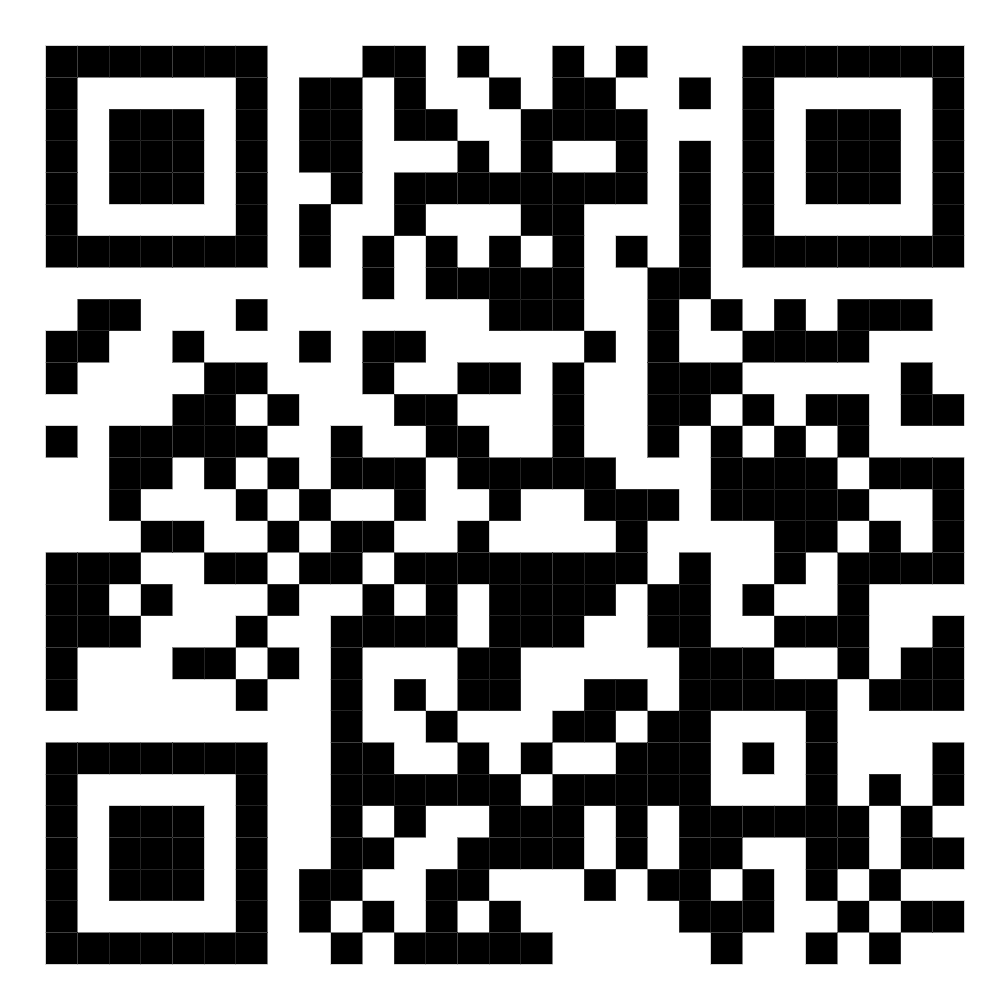
\includegraphics[width=0.3\textwidth]{qr.png} 
	
	% Hoặc dùng gói qrcode để tự sinh
	% \qrcode[height=3cm]{https://github.com/lehuynhanhkhoi/cryptography-project}
	
	\caption{Mã nguồn tại \href{https://github.com/itsanhkhoi12/infor-sec-uth-2026}{Github}}
	\label{fig:qr_code}
\end{figure}

% Minh chứng thực hiện code
